%\documentclass[final,hyperref={pdfpagelabels=false}]{beamer}
\documentclass[final]{beamer}
\usepackage{grffile}
%\mode<presentation>{\usetheme{Singapore}}
\mode<presentation>{\usetheme{I6pd2}}
\usepackage[english]{babel}
%\usepackage[latin1]{inputenc}
\usepackage[utf8]{inputenc}
\usepackage{amsmath,amsthm, amssymb, latexsym}
%\usepackage{times}\usefonttheme{professionalfonts}  % obsolete
%\usefonttheme[onlymath]{serif}
\boldmath
\usepackage[orientation=portrait,size=a0,scale=1.4,debug]{beamerposter}
% change list indention level
% \setdefaultleftmargin{3em}{}{}{}{}{}

%\setbeamercolor{structure}{fg=ta3skyblue}

%\usepackage{snapshot} % will write a .dep file with all dependencies, allows for easy bundling

\usepackage{array,booktabs,tabularx}
\newcolumntype{Z}{>{\centering\arraybackslash}X} % centered tabularx columns
\newcommand{\pphantom}{\textcolor{ta3aluminium}} % phantom introduces a vertical space in p formatted table columns??!!

\listfiles

%%%%%%%%%%%%%%%%%%%%%%%%%%%%%%%%%%%%%%%%%%%%%%%%%%%%%%%%%%%%%%%%%%%%%%%%%%%%%%%%%%%%%%
\graphicspath{{figures/}}
 
\title{\huge Towards a Cognitive Monitoring BCI application for Assitive Robotics}
\author{Santos Juan Miguel, Villar Ana Julia,  Ramele Rodrigo}
\institute[Instituto Tecnológico de Buenos Aires]{Computer Engineering Department,Graduate School in Engineering, Buenos Aires, Argentina}
\date[Aug. 26th, 2013]{Aug. 26th, 2013}

%%%%%%%%%%%%%%%%%%%%%%%%%%%%%%%%%%%%%%%%%%%%%%%%%%%%%%%%%%%%%%%%%%%%%%%%%%%%%%%%%%%%%%
\newlength{\columnheight}
\setlength{\columnheight}{105cm}


%%%%%%%%%%%%%%%%%%%%%%%%%%%%%%%%%%%%%%%%%%%%%%%%%%%%%%%%%%%%%%%%%%%%%%%%%%%%%%%%%%%%%%
\begin{document}
\begin{frame}

  \begin{columns}
    % ---------------------------------------------------------%
    % Set up a column 
    \begin{column}{.49\textwidth}       
            \begin{block}{Introduction}
              \begin{itemize}
              \item \textbf{Brain Computer Interfaces Research is becoming a mature discipline.}
                \begin{itemize}
                \item Through the last fifteen years, many successful projects have proved the practicability of the technology to transfer information from the Central Nervous System to a computer
                \end{itemize}
              \item \textbf{BCIs are now being considered an important branch of HCI (Human Computer Interaction).}
                \begin{itemize}
                \item The ability to combine multiple bio-channels together, the so called hBCI (Hybrid BCI), in order to transmit more information, is quickly expanding the uses of these devices to many more useful niches as HCI.
                \end{itemize}
              \item Although, this widespread usage, the key aspect of BCI still lies in its support into \textbf{Assitive Technologies}.   
                \begin{itemize}
                \item Passive Technology is pushing the boundaries of Robotics environments from industrial applications and constrained laboratories  into the common ground of real world applications where humans develop their daily activities. 
                \item By merging these technologies, we aim to develop a hBCI-enhanced  Passive Walking Helper device with a direct application in gerontology. 
                \end{itemize}
              \end{itemize}               
            \end{block}
            \vfill
    \end{column}
    % ---------------------------------------------------------%
    % end the column

    % ---------------------------------------------------------%
    % Set up a column 
    \begin{column}{.49\textwidth}            
            \begin{block}{Motivations}
              \begin{columns}
                \begin{column}{.6\textwidth}
                  \begin{itemize}
                  \item Aging Societies
                    \begin{itemize}
		    \item Estimated for 2025, 800 millions people will be over 65 old.
                    \item 2/3 of them on ''developing'' countries.
                    \end{itemize}
                  \item Through technology, provide a better quality of life for more people.
                    \begin{itemize}
                    \item Specially for those affected by diseases or disabilities.
                    \end{itemize}
                  \item Active lifestyle: enhance mobility.
                    \begin{itemize}
                    \item Ability to walk independently is a key indicator of psychological and physical health. 
                    \end{itemize}
                  \item Digital World demands more methods of interactions.
                    \begin{itemize}
                    \item We need more mechanisms to interpret our surrounding world and to translate our intentions through our digital gadgets.
                    \end{itemize}
                  \end{itemize}
                \end{column}
                \begin{column}{.39\textwidth}
		    \centering
		    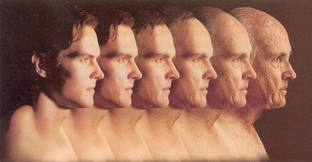
\includegraphics[width=0.95\linewidth]{images/viola/aging}
\-
                    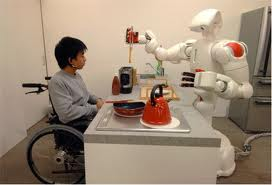
\includegraphics[width=0.95\linewidth]{images/viola/disabilities}
\-                                                                                  
		    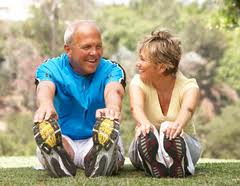
\includegraphics[width=0.95\linewidth]{images/viola/exercise}
\-
                \end{column}
              \end{columns}
            \end{block}

    \end{column}
    % ---------------------------------------------------------%
    % end the column
  \end{columns}
  
            \begin{block}{Work in Progress}
              \begin{itemize}
              \item \textbf{Research Questions}
                \begin{itemize}
                \item Is it possible to achieve a faster BCI scheme by centering on the feedback from the real environment ?
                \item Does a BCI-powered assistive device allows better controllability and maneuverability?
                \item Is it possible to use Passive BCI (e.g. without user awareness) to enhance the safety of an assistive walking device ?
                \end{itemize}
              \end{itemize}  
		\centering
                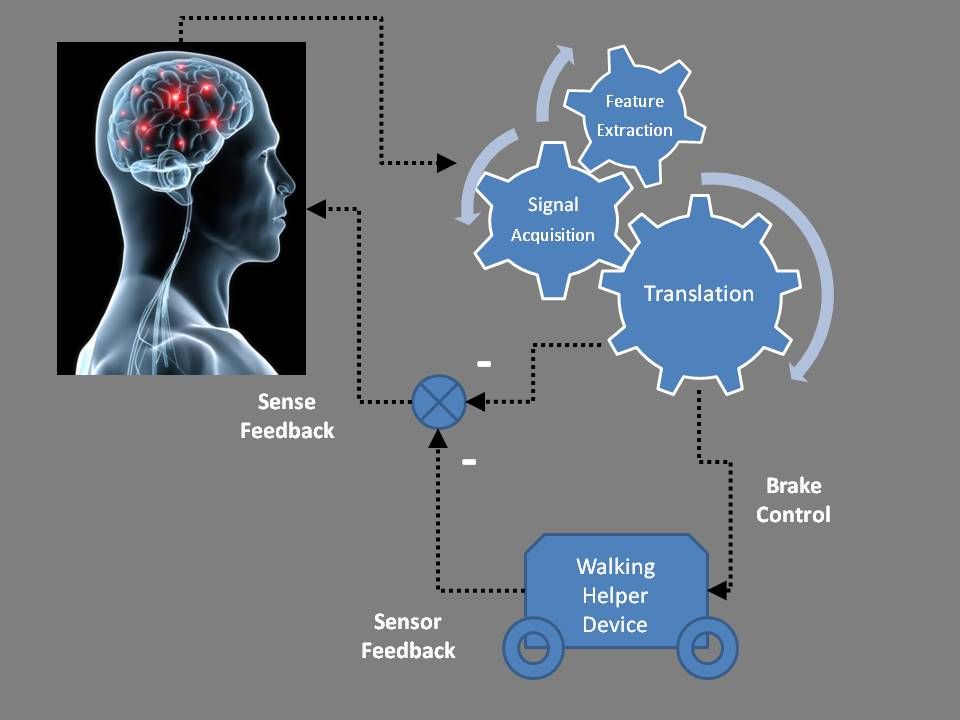
\includegraphics[width=0.4\linewidth]{images/viola/bcidesign}
            \end{block}
  
  
  
  
  \begin{columns}
    % ---------------------------------------------------------%
    % Set up a column 
    \begin{column}{.49\textwidth}
            \vfill
            \begin{block}{Visual Spatial Covert Attention and $ \alpha$  waves}
              \begin{itemize}
              \item Metodos como fue que se hizo este experimento.  Explicar en el cuadro de arriba por que se usa este metodo.
              
		\centering
                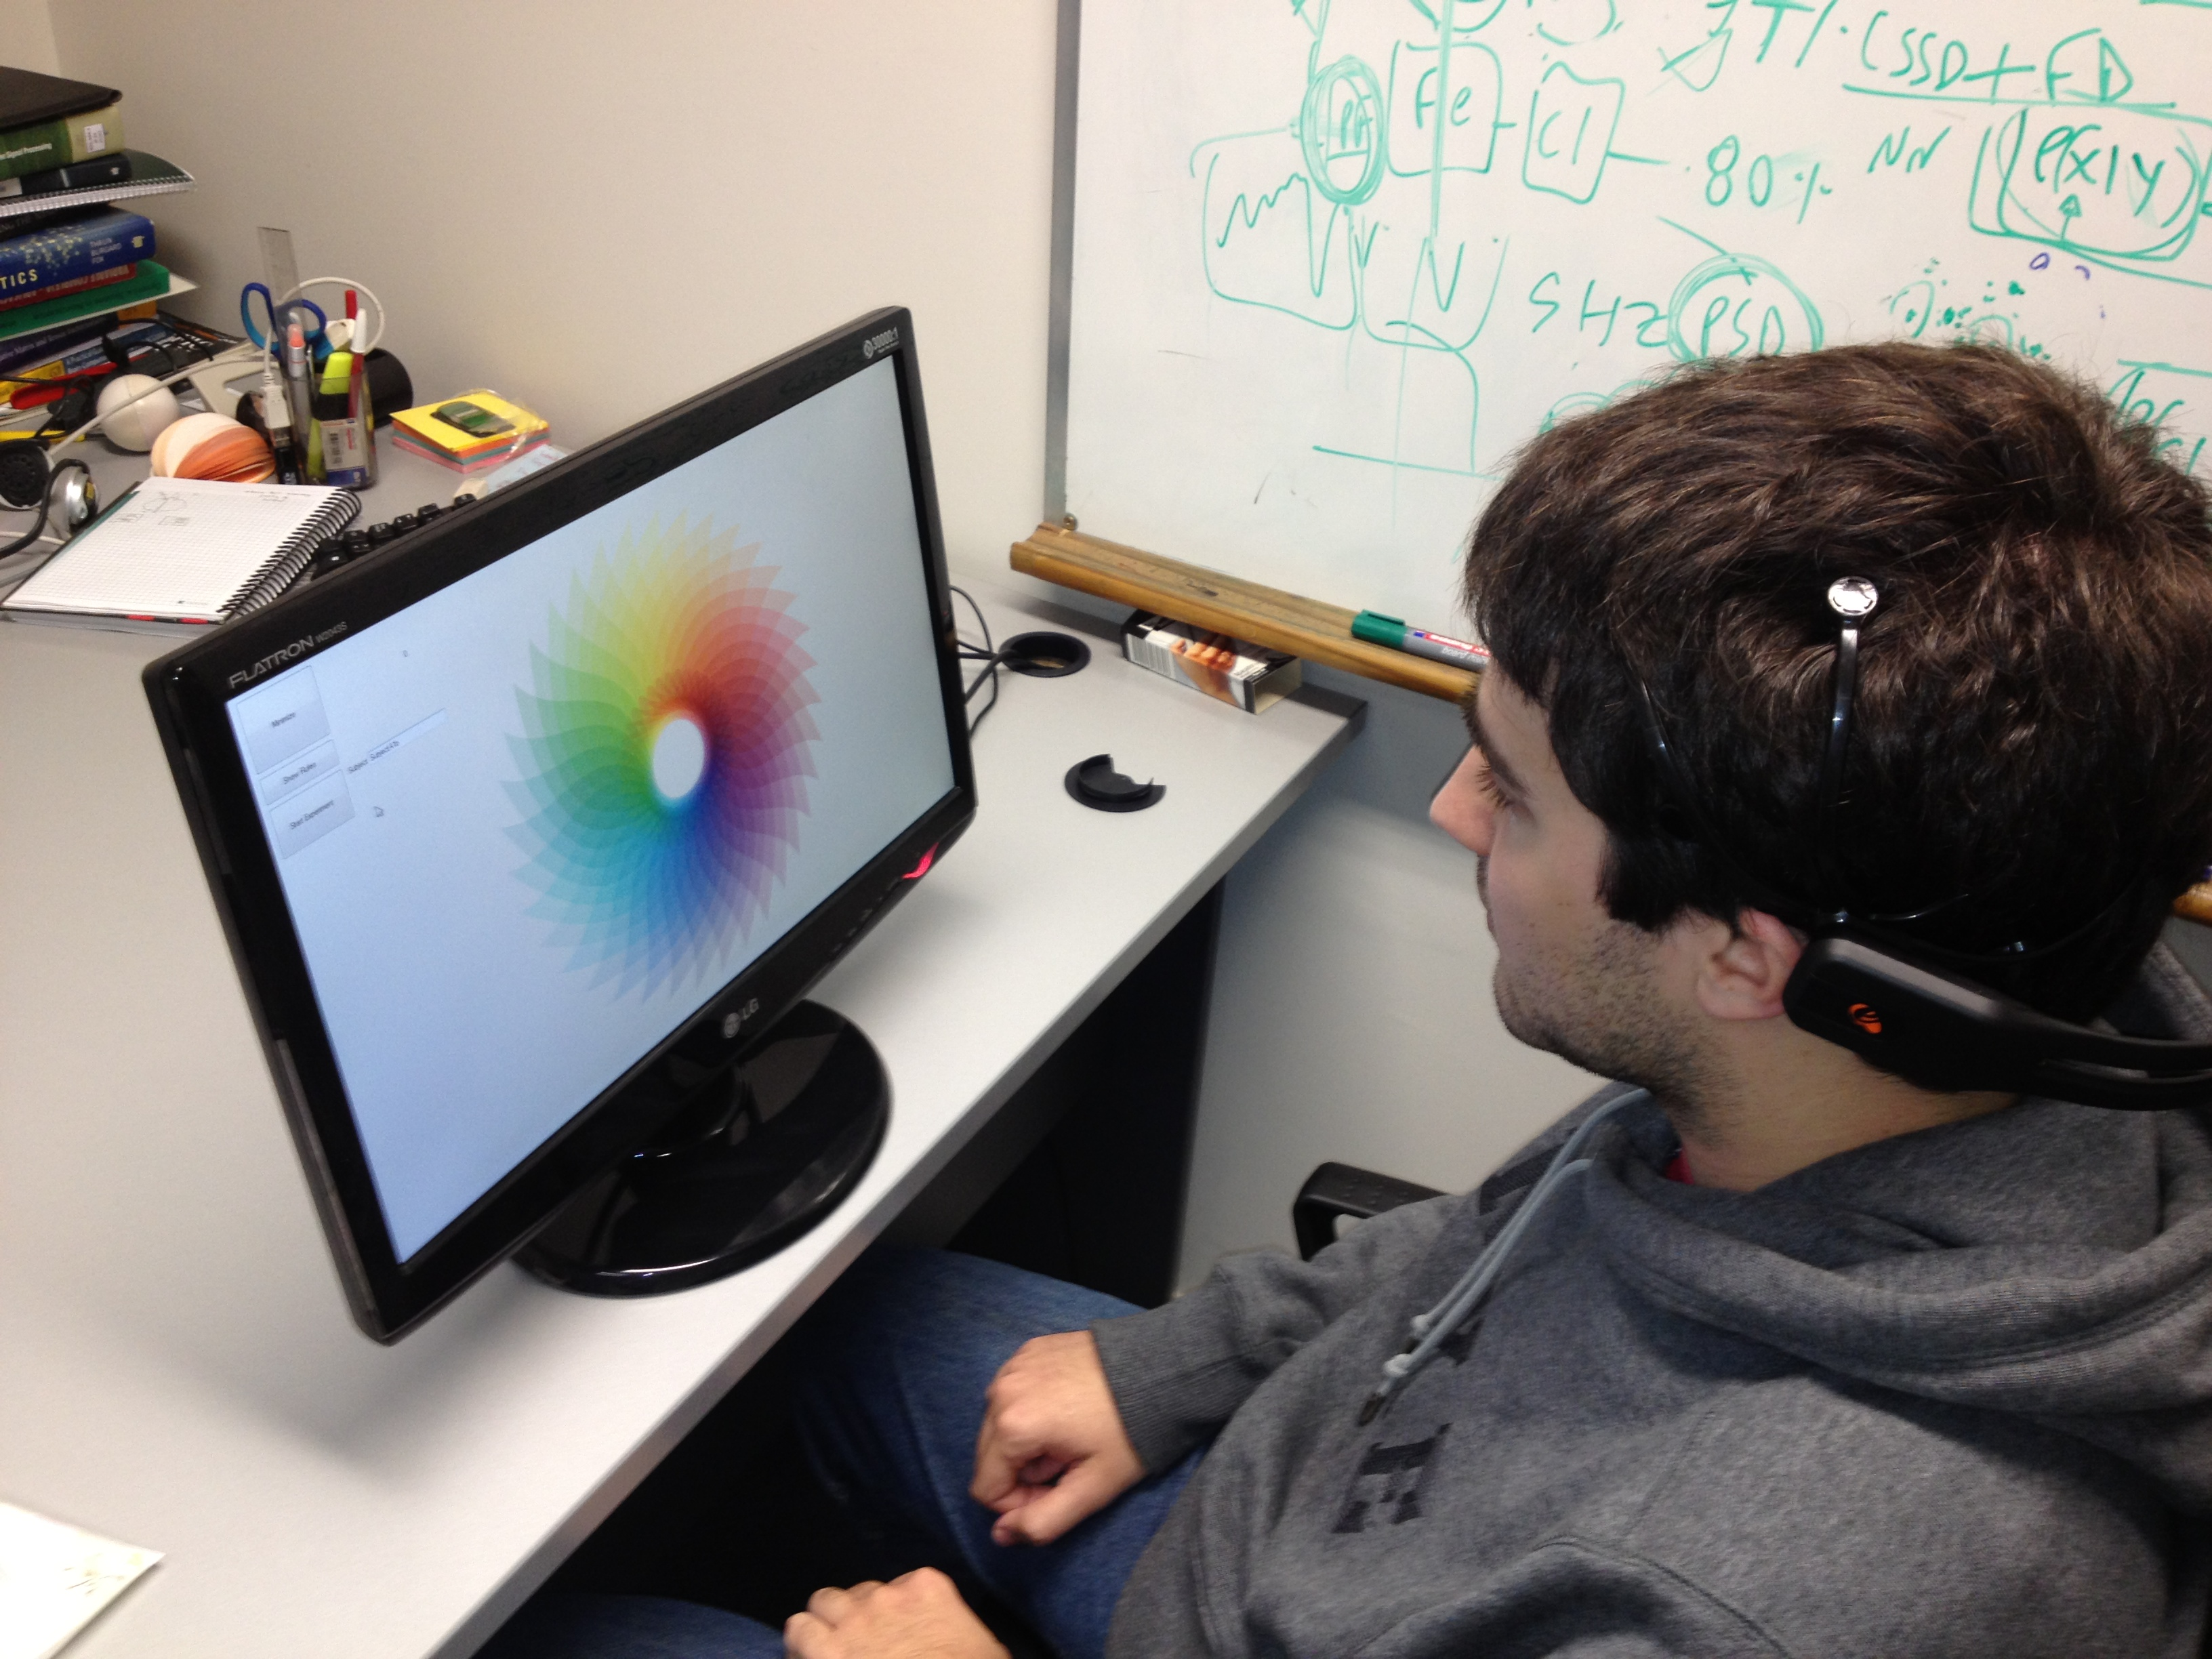
\includegraphics[width=0.80\linewidth]{images/viola/subject}
			       \item User gaze centered on the image.
                \begin{itemize}
                \item Flickering light on both sides of the screen at different frequency rates.
                \item Common Spatial Patterns and CSSD
                  \begin{align*}
		    \mathbf{M} \Delta \ddot{x} + \mathbf{D} \Delta \dot{x} + \mathbf{K} \Delta x = \mathbf{F}
                  \end{align*}
                \item Stability considerations (Desoer and Kuh, 1969)
                \item Low Energy Consumption.
                \item Passive Dynamics (motor-less walking bipeds). 
                \end{itemize}

              \end{itemize}
            \end{block}
                          \vfill

            
%                        \begin{block}{Embodied Assistive Robotics}
%              \begin{columns}
%                \begin{column}{.55\textwidth}
%                  \begin{itemize}
%                  \item Incluir un buen dibujo que resuma todo el proceso de embodiement.
%                  \item Where is this signal ?  Can be seen from a noninvsaive EEG ?
%                  \item Is it possible to use this signal to modulate information ?
%                  \item Sense human intentions. Awareness of common elements in human environment.
%                  \item Real World Applications
%                    \begin{itemize}
%                    \item Environments are unpredictable
%                    \item Sensors are limited
%                    \item Sensors are unreliable
%                    \item Actuation is imprecise
%                    \item Models are approximate
%                    \item Algorithms are approximate
%                    \end{itemize}
%                  \end{itemize}
%                \end{column}
%                \begin{column}{.44\textwidth}
%                  \centering
%                    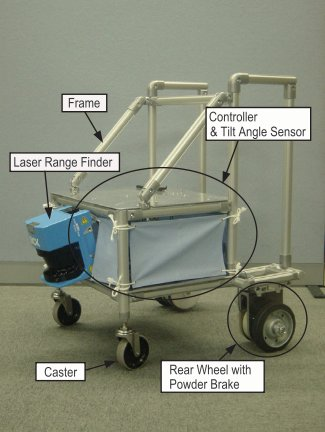
\includegraphics[width=0.95\linewidth]{images/viola/rtwalkernew}
%                \end{column}
%              \end{columns}
%              \vskip-1ex
%            \end{block}
            
    \end{column}
    % ---------------------------------------------------------%
    % end the column

    % ---------------------------------------------------------%
    % Set up a column 
    \begin{column}{.49\textwidth}

            \begin{block}{Objective: Encourage Locomotion Independence and Improve Rehabilitation Practices}
	      \begin{itemize}
                 
                  \item Implement a Robotic Walking Device to assist persons with partial walking disabilities.
                  \item Use of hybrid BCI to enhance an assistive robotic device in order to move safely and effectively through a non-constrained environment.
                 
                  \item Brain Computer Interface 
                
                  \begin{itemize}
                  \item Online - Non-Invasive - Asynchronous.
                  \item Electroencephalogram.
                  \item Wearable
                  \item Mutual Interactive of Adaptive Controllers Approach.
                  \item BCI2000/OpenVibe: Reuse and contribute (\textit{support community open source software!})
                  \end{itemize}
                 
                  \item Hybrid-BCI
                
                  \begin{itemize}
                  \item Use of EMG and correlate it with EEG input signal.
                  \item Sensor Fusion: Force-Sensor, Inertial, Ultrasonic ranger.
                  \end{itemize}

                  %\item Apply Q-Learning techniques to the solution of the EEG inverse problem.
                  
	      \end{itemize}
            \end{block}
            \vfill

            \begin{block}{References and Previous Works}
              \begin{itemize}
                \item \small A. Cherubini, G. Oriolo, F. Macri, F. Aloise, F. Babiloni, F. Cincotti, and D. Mattia. Development of a
multimode navigation system for an assistive robotics project. \textit{Proceedings 2007 IEEE International
Conference on Robotics and Automation}, pages 2336–2342, April 2007.
                \item F Galan, M Nuttin, E Lew, P W Ferrez, G Vanacker, J Philips, and J Del R Millan. A brain-actuated
wheelchair: asynchronous and non-invasive Brain-computer interfaces for continuous control of robots.
\textit{Clinical neurophysiology : official journal of the International Federation of Clinical Neurophysiology},
119(9):2159–69, September 2008.
                \item Yasuhisa Hirata, Shinji Komatsuda, and Kazuhiro Kosuge. Fall prevention control of passive intelligent
walker based on human model. \textit{2008 IEEE/RSJ International Conference on Intelligent Robots and
Systems}, pages 1222–1228, September 2008.
                \item Tan Desney S.  (Editor), Nijholt Anton (Editor)  et al, \textit{Brain-Computer Interfaces: Applying our minds to Human-Computer Interaction},2010, Springer
              \end{itemize}

            \end{block}
            \vfill
    \end{column}
    % ---------------------------------------------------------%
    % end the column
  \end{columns}
  \vskip1ex
  %\tiny\hfill\textcolor{ta2gray}{Created with \LaTeX \texttt{beamerposter}  \url{http://www-i6.informatik.rwth-aachen.de/~dreuw/latexbeamerposter.php}}
  \tiny\hfill{Created with \LaTeX \texttt{beamerposter}  \url{http://www-i6.informatik.rwth-aachen.de/~dreuw/latexbeamerposter.php} \hskip1em}
\end{frame}
\end{document}


%%%%%%%%%%%%%%%%%%%%%%%%%%%%%%%%%%%%%%%%%%%%%%%%%%%%%%%%%%%%%%%%%%%%%%%%%%%%%%%%%%%%%%%%%%%%%%%%%%%%
%%% Local Variables: 
%%% mode: latex
%%% TeX-PDF-mode: t
%%% End:
